\documentclass[12pt,titlepage,a4page , tikz , multi,table , svgnames,xcdraw]{article}
\usepackage{graphicx}
\usepackage[svgnames , table , xcdraw]{xcolor} 
\usepackage{fancyhdr}
 
\usepackage{hyperref}
\hypersetup{
    colorlinks=true,
    linkcolor=blue,
    filecolor=magenta,      
    urlcolor=cyan,
}

\usepackage{mathtools}
\usepackage{multirow}
\usepackage{graphicx}
\usepackage{float}
\usepackage{enumitem}
\usepackage{listings }
\usepackage[a4paper, total={6in, 8in}]{geometry}
\usepackage{afterpage}
\usepackage{amssymb}
\usepackage{pdflscape}
\usepackage{lscape}
\usepackage{amsmath}
\usepackage{svg}
\usepackage[final]{pdfpages}

\usepackage{pgf, tikz}
\usetikzlibrary{arrows, automata}
\usetikzlibrary{shapes.multipart}


\usepackage[T1]{fontenc}
\usepackage{tikz}
\usepackage[utf8]{inputenc} % Required for inputting international characters
\usepackage{PTSerif} 

\usepackage{float}

\usepackage[Kashida]{xepersian}
\settextfont[
 BoldFont={XB NiloofarBd.ttf}
 ]{XB Niloofar.ttf}


\NewDocumentCommand{\codeword}{v}{
\texttt{\textcolor{blue}{#1}}
}
\DeclareFixedFont{\ttb}{T1}{txtt}{bx}{n}{12} % for bold
\DeclareFixedFont{\ttm}{T1}{txtt}{m}{n}{12}  % for normal


\definecolor{deepblue}{rgb}{0,0,0.5}
\definecolor{deepred}{rgb}{0.6,0,0}
\definecolor{deepgreen}{rgb}{0,0.5,0}

\newcommand\independent{\protect\mathpalette{\protect\independenT}{\perp}}
\def\independenT#1#2{\mathrel{\rlap{$#1#2$}\mkern2mu{#1#2}}}

% Python style for highlighting
\newcommand\pythonstyle{\lstset{
language=Python,
basicstyle=\ttm,
otherkeywords={self},             % Add keywords here
keywordstyle=\ttb\color{deepblue},
emph={MyClass,__init__},          % Custom highlighting
emphstyle=\ttb\color{deepred},    % Custom highlighting style
stringstyle=\color{deepgreen},
frame=tb,                         % Any extra options here
showstringspaces=false            % 
}}


% Python environment
\lstnewenvironment{python}[1][]
{
\pythonstyle
\lstset{#1}
}
{}

% Python for external files
\newcommand\pythonexternal[2][]{{
\pythonstyle
\lstinputlisting[#1]{#2}}}

\newenvironment{changemargin}[2]{%
\begin{list}{}{%
\setlength{\topsep}{0pt}%
\setlength{\leftmargin}{#1}%
\setlength{\rightmargin}{#2}%
\setlength{\listparindent}{\parindent}%
\setlength{\itemindent}{\parindent}%
\setlength{\parsep}{\parskip}%
}%
\item[]}{\end{list}}

% Python for inline
\newcommand\pythoninline[1]{{\pythonstyle\lstinline!#1!}}


\begin{document}

\begin{titlepage}

 \begin{center}
        
       \vspace*{1cm}

 \vspace{1cm}
       \textbf{ \Huge{به نام خدا} }
       \vspace{0.4cm}
       
       
\includegraphics[width=0.4\textwidth]{sharif.png}
       
 	\vspace{0.7cm}
       \textbf{ \LARGE{معماری کامپیوتر} }

 
   \vspace{0.7cm}
  \textbf{ \Large{ پروژهٔ پایانی - بخش دوم - شبیه‌سازی \lr{gem5}} }
   \vspace{0.5cm}
       
 
      \large \textbf{دانشکدهٔ مهندسی کامپیوتر}\\\vspace{0.2cm}
    \large   دانشگاه صنعتی شریف\\\vspace{0.25cm}
      
استاد:\\
    \textbf{{جناب آقای دکتر اسدی}}

    \vspace{0.15cm}
    \noindent\rule[1ex]{\linewidth}{3pt}
    
    \vspace{0.5cm}
نام، نام خانوادگی و شمارهٔ دانشجویی اعضای گروه:\\
    \textbf{{سپهر پورقناد - 97101359}}
        \vspace{0.1cm}
        
     \textbf{{سیدمحمدصادق کشاورزی - 97106249}}
        \vspace{0.1cm}
        
       \textbf{{امیرمهدی نامجو - 97107212}}
        \vspace{0.1cm}


\end{center}
\end{titlepage}

\newpage
\pagestyle{fancy}
\fancyhf{}
\fancyfoot{}

\cfoot{\thepage}
\chead{پروژهٔ پایانی}
\rhead{شبیه‌ساز \lr{gem5}}
\lhead{معماری کامپیوتر}

\newpage
\section{بررسی دستورات}
الگوریتم
\lr{SHA-256}
دارای دو دسته از دستورات است که به صورت دستورات رایج
\lr{ISA}
نیست. در واقع این دستورات ترکیبی از چند دستور رایج
\lr{ISA}
هستند که مقادیر محاسبه‌شدهٔ میانی دوباره استفاده نمی‌شوند. اگر هر کدام از این دستورات را بتوان در مدت زمان یک دستور رایج
\lr{ISA}
انجام داد، سرعت اجرای برنامه سریع‌تر می‌شود. این دو دسته به صورت زیر هستند:
\par
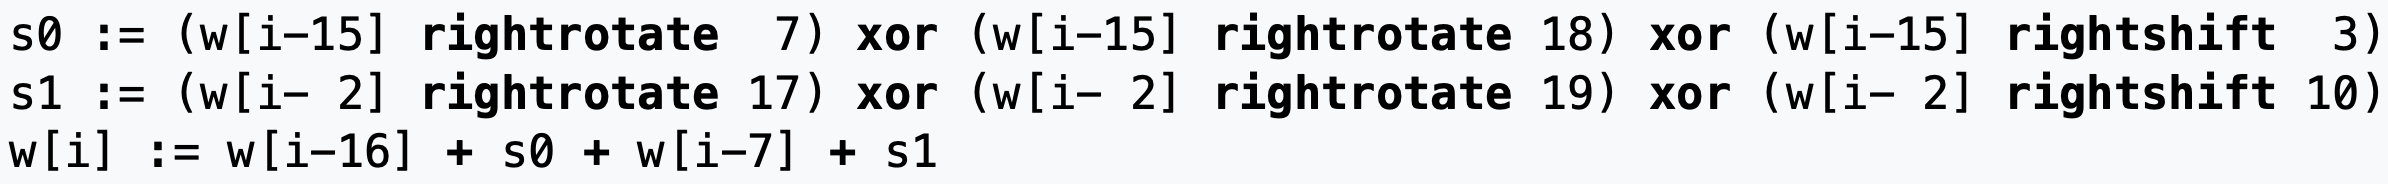
\includegraphics[width=\textwidth]{1.png}
\par
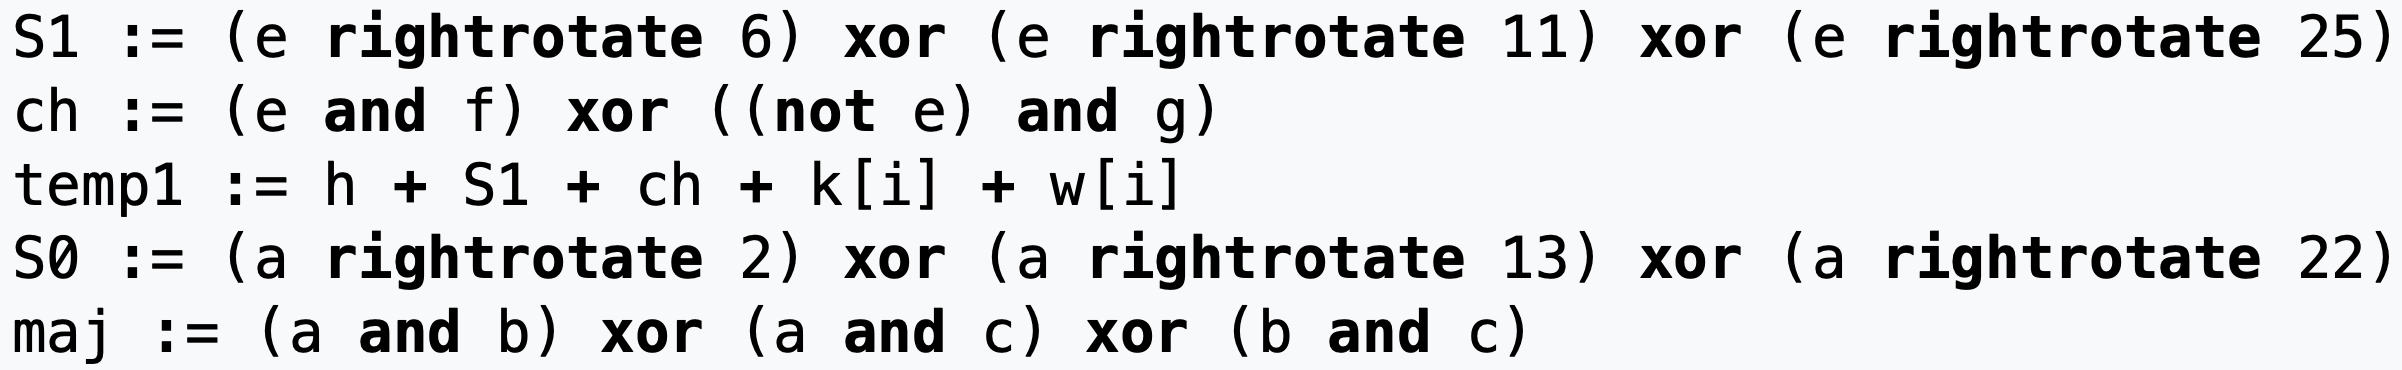
\includegraphics[width=\textwidth]{2.png}
\par
هر کدام از دستورات بالا گزینه‌ای برای اضافه کردن به
\lr{ISA}
است. ما در اینجا دستور\\
\lr{\texttt{a = (b \& c) \^{} (\textasciitilde b \& d)}}
پیاده‌سازی می‌کنیم و اثر آن بر بهبود سرعت اجرای برنامه را بررسی می‌کنیم.
\newpage
\section{اضافه کردن دستور}
فایل
\lr{\texttt{src/arch/x86/isa/decoder/two\_byte\_opcodes.isa}}:
\par
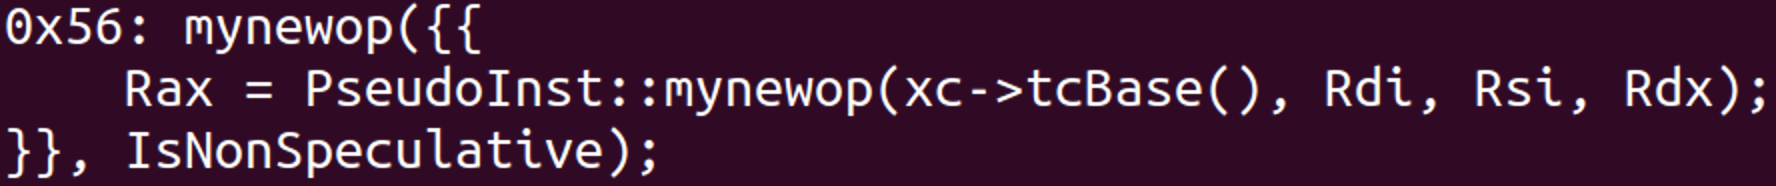
\includegraphics[width=\textwidth]{3.png}
\par
فایل
\lr{\texttt{src/sim/pseudo\_inst.cc}}:
\par
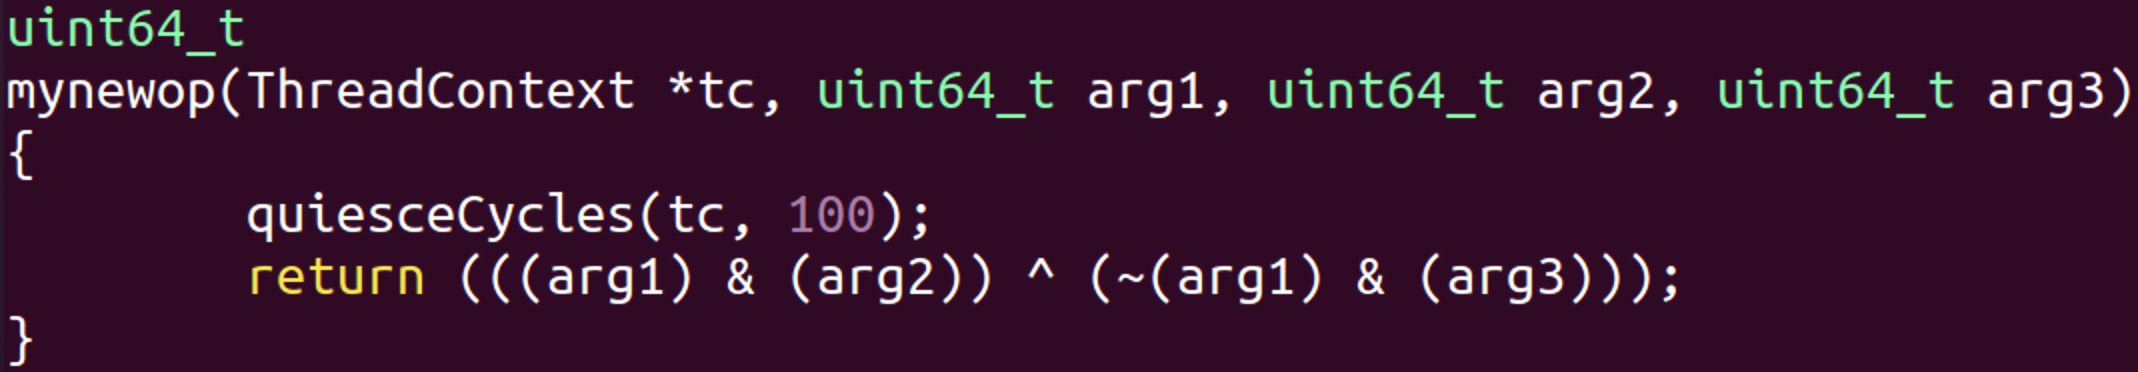
\includegraphics[width=\textwidth]{4.png}
\par
که تأخیر اجرای دستور را (بر حسب تعداد چرخهٔ ساعت) به عنوان ورودی به دستور
\lr{\texttt{quiesceCycle}}
می‌دهیم (که در مثال بالا برابر ۱۰۰ چرخهٔ ساعت است).
\par
۳ تأخیر زیر را برای این دستور در نظر می‌گیریم:
\begin{enumerate}
\item
۱ چرخهٔ ساعت: که حالت ایده‌آل است.
\item
۲۰ چرخهٔ ساعت: که برابر تعداد چرخهٔ لازم برای اجرای این دستور در پردازندهٔ
\lr{multicycle}
آموزش‌داده‌شده در درس است (با فرض موجود بودن متغیرها در ثبات‌ها).
\item
۱۰۰ چرخهٔ ساعت: که تخمینی برای حد بالای تعداد چرخهٔ لازم برای اجرای این دستور در پردازندهٔ ۸۰۸۶ است (با فرض موجود بودن متغیرها در حافظه).
\end{enumerate}
زمان‌های اجرا به ازای رشتهٔ ورودی
\lr{"how are you doing today?"}
 به شرح زیر است:
\begin{enumerate}
\item
\lr{ISA}
اصلی: ۱۶۳٬۰۲۱٬۰۰۰ تیک
\item
دستور اختصاصی با تأخیر ۱ چرخهٔ ساعت: ۱۶۳٬۴۶۰٬۰۰۰ تیک
$\leftarrow$
بهبود = ۰٫۹۹۷ (احتمالاً علت این که نه تنها بهبود نداشته‌ایم، بلکه زمان اجرا بدتر نیز شده‌است، این است که کامپایلر این دستور را نمی‌شناسد و اجرای این دستور جدید، بهینه‌سازی‌های کامپایلر (از جمله تخصیص ثبات) را به هم می‌ریزد و از بین می‌برد).
\item
دستور اختصاصی با تأخیر ۲۰ چرخهٔ ساعت: ۱۶۴٬۰۶۸٬۰۰۰ تیک
$\leftarrow$
بهبود = ۰٫۹۹۳
\item
دستور اختصاصی با تأخیر ۱۰۰ چرخهٔ ساعت: ۳۲٬۱۶۳٬۴۲۸٬۰۰۰ تیک
$\leftarrow$
بهبود = ۰٫۰۰۵۰۶
\end{enumerate}
همهٔ حالات با تنظیمات
\lr{\texttt{se.py}}
بدون هیچ تغییری اجرا شدند و هر ثانیه برابر
$10^{12}$
تیک است.
\newpage
\section{تأثیر حافظهٔ نهان}
\begin{itemize}
\item
\lr{ISA}
اصلی:
\begin{itemize}
\item
بدون حافظهٔ نهان: ۱۳٬۲۸۸٬۷۳۰٬۰۰۰ تیک
\item
حافظهٔ نهان دوسطحی: ۷۳۵٬۴۷۴٬۰۰۰ تیک
$\leftarrow$
بهبود = ۱۸٫۰۶۸
\end{itemize}
تعداد دسترسی‌های خواندن‌ داده از حافظه از ۴۵۰۵۲ به ۴۵۰۴۶ و نوشتن دستور به حافظه از ۱۹۹۸۴۳ به ۱۹۹۷۵۶ کاهش یافته‌است. تعداد دسترسی‌ها و
\lr{miss}های
دیگر تغییر نداشته‌است.
\item
دستور اختصاصی با تأخیر ۱۰۰ چرخهٔ ساعت:
\begin{itemize}
\item
بدون حافظهٔ نهان: ۱۳٬۳۳۲٬۸۹۴٬۰۰۰
\item
حافظهٔ نهان دوسطحی: ۷۴۲٬۸۴۳٬۰۰۰
$\leftarrow$
بهبود = ۱۷٫۹۴۸
\end{itemize}
تعداد خواندن‌های داده از حافظه نیز از ۴۵۰۵۲ به ۴۵۰۴۶ و تعداد نوشتن‌های دستور به حافظه از ۲۰۰۶۳۴ به ۲۰۰۵۴۷ کاهش یافته‌است. تعداد دسترسی‌ها و
\lr{miss}های
دیگر تغییر نداشته‌است.
\end{itemize}
\newpage
\section{تنظیمات حافظهٔ نهان}
اثر پارامترهای مختلف بر کارایی برنامه را در حالت استفاده از دستور اختصاصی با تأخیر ۱۰۰ چرخهٔ ساعت بررسی می‌کنیم:
\begin{itemize}
\item
بدون تغییرات: ۷۴۲٬۸۴۳٬۰۰۰ تیک (در این حالت
\lr{associativity}
برابر ۶۴ است.)
\item
\lr{Cacheline}:
\begin{itemize}
\item
۳۲: ۸۷۳٬۷۷۹٬۰۰۰
$\leftarrow$
بهبود = ۰٫۸۵۰
\item
۶۴: ۷۸۲٬۸۴۳٬۰۰۰؛
احتمالاً مقدار از پیش تعیین‌شدهٔ این پارامتر در سیستم همین مقدار است و به همین علت هیچ بهبودی مشاهده نمی‌شود.
\end{itemize}
\item
\lr{L2 Cache Associativity}:
\begin{itemize}
\item
۸: ۷۴۲٬۸۴۳٬۰۰۰
\item
۱۶: ۷۴۲٬۸۴۳٬۰۰۰
\end{itemize}
در واقع در اجراهای مختلف مشاهده شد که زمان اجرا به ازای مقادیر مختلف این پارامتر به غیر از ۱ با یکدیگر برابر هستند، که احتمالاً به علت کم بودن تعداد برخوردها در حافظهٔ نهان است. به طور کلی تقریباً همهٔ آمار و ارقام مربوط به دو مقدار متفاوت
\lr{associativity}
با یکدیگر برابر بودند که احتمالاً به دلیل تعداد کم متغیرهای موجود در برنامه، و تکرار عملیات یکسان در طی اجرا است.
\end{itemize}
\end{document}












